%%%%%%%%%%%%%%%%%%%%%%%%%%%%%%%%%%%%%%%%%
% Proceedings of the National Academy of Sciences (PNAS)
% LaTeX Template
% Version 1.0 (19/5/13)
%
% This template has been downloaded from:
% http://www.LaTeXTemplates.com
%
% Original author:
% The PNAStwo class was created and is owned by PNAS:
% http://www.pnas.org/site/authors/LaTex.xhtml
% This template has been modified from the blank PNAS template to include
% examples of how to insert content and drastically change commenting. The
% structural integrity is maintained as in the original blank template.
%
% Original header:
%% PNAStmpl.tex
%% Template file to use for PNAS articles prepared in LaTeX
%% Version: Apr 14, 2008
%
%%%%%%%%%%%%%%%%%%%%%%%%%%%%%%%%%%%%%%%%%

%----------------------------------------------------------------------------------------
%	PACKAGES AND OTHER DOCUMENT CONFIGURATIONS
%----------------------------------------------------------------------------------------

%------------------------------------------------
% BASIC CLASS FILE
%------------------------------------------------

%% PNAStwo for two column articles is called by default.
%% Uncomment PNASone for single column articles. One column class
%% and style files are available upon request from pnas@nas.edu.

%\documentclass{pnasone}
\documentclass{pnastwo}

%------------------------------------------------
% POSITION OF TEXT
%------------------------------------------------

%% Changing position of text on physical page:
%% Since not all printers position
%% the printed page in the same place on the physical page,
%% you can change the position yourself here, if you need to:

% \advance\voffset -.5in % Minus dimension will raise the printed page on the 
                         %  physical page; positive dimension will lower it.

%% You may set the dimension to the size that you need.

%------------------------------------------------
% GRAPHICS STYLE FILE
%------------------------------------------------

%% Requires graphics style file (graphicx.sty), used for inserting
%% .eps/image files into LaTeX articles.
%% Note that inclusion of .eps files is for your reference only;
%% when submitting to PNAS please submit figures separately.

%% Type into the square brackets the name of the driver program 
%% that you are using. If you don't know, try dvips, which is the
%% most common PC driver, or textures for the Mac. These are the options:

% [dvips], [xdvi], [dvipdf], [dvipdfm], [dvipdfmx], [pdftex], [dvipsone],
% [dviwindo], [emtex], [dviwin], [pctexps], [pctexwin], [pctexhp], [pctex32],
% [truetex], [tcidvi], [vtex], [oztex], [textures], [xetex]

\usepackage{graphicx}

%------------------------------------------------
% OPTIONAL POSTSCRIPT FONT FILES
%------------------------------------------------

%% PostScript font files: You may need to edit the PNASoneF.sty
%% or PNAStwoF.sty file to make the font names match those on your system. 
%% Alternatively, you can leave the font style file commands commented out
%% and typeset your article using the default Computer Modern 
%% fonts (recommended). If accepted, your article will be typeset
%% at PNAS using PostScript fonts.

% Choose PNASoneF for one column; PNAStwoF for two column:
%\usepackage{PNASoneF}
%\usepackage{PNAStwoF}

%------------------------------------------------
% ADDITIONAL OPTIONAL STYLE FILES
%------------------------------------------------

%% The AMS math files are commonly used to gain access to useful features
%% like extended math fonts and math commands.

\usepackage{amssymb,amsfonts,amsmath}
\usepackage[]{algorithm2e}

%------------------------------------------------
% OPTIONAL MACRO FILES
%------------------------------------------------

%% Insert self-defined macros here.
%% \newcommand definitions are recommended; \def definitions are supported

%\newcommand{\mfrac}[2]{\frac{\displaystyle #1}{\displaystyle #2}}
%\def\s{\sigma}

%------------------------------------------------
% DO NOT EDIT THIS SECTION
%------------------------------------------------

%% For PNAS Only:
\contributor{CS289, Harvard University}
\url{Wang and Zhang}
\copyrightyear{2014}
\volume{Spring}
\issuedate{}
\issuenumber{}

%----------------------------------------------------------------------------------------

\begin{document}

%----------------------------------------------------------------------------------------
%	TITLE AND AUTHORS
%----------------------------------------------------------------------------------------

\title{Genetic Algorithms in Painting} % For titles, only capitalize the first letter

%------------------------------------------------

%% Enter authors via the \author command.  
%% Use \affil to define affiliations.
%% (Leave no spaces between author name and \affil command)

%% Note that the \thanks{} command has been disabled in favor of
%% a generic, reserved space for PNAS publication footnotes.

%% \author{<author name>
%% \affil{<number>}{<Institution>}} One number for each institution.
%% The same number should be used for authors that
%% are affiliated with the same institution, after the first time
%% only the number is needed, ie, \affil{number}{text}, \affil{number}{}
%% Then, before last author ...
%% \and
%% \author{<author name>
%% \affil{<number>}{}}

%% For example, assuming Garcia and Sonnery are both affiliated with
%% Universidad de Murcia:
%% \author{Roberta Graff\affil{1}{University of Cambridge, Cambridge,
%% United Kingdom},
%% Javier de Ruiz Garcia\aff	il{2}{Universidad de Murcia, Bioquimica y Biologia
%% Molecular, Murcia, Spain}, \and Franklin Sonnery\affil{2}{}}

\author{Andrew Wang\affil{1}{awang@college.harvard.edu}
\and
Kevin Zhang\affil{2}{kzhang@college.harvard.edu}}

\contributor{Computer Science 289 Final Project}

%----------------------------------------------------------------------------------------

\maketitle % The \maketitle command is necessary to build the title page

\begin{article}

%----------------------------------------------------------------------------------------
%	ABSTRACT, KEYWORDS AND ABBREVIATIONS
%----------------------------------------------------------------------------------------

\begin{abstract}
ABSTRACT
\end{abstract}

%------------------------------------------------

\keywords{Genetic Algorithms | Image Processing | Hill Climbing} % When adding keywords, separate each term with a straight line: |

%------------------------------------------------

%% Optional for entering abbreviations, separate the abbreviation from
%% its definition with a comma, separate each pair with a semicolon:
%% for example:
%% \abbreviations{SAM, self-assembled monolayer; OTS,
%% octadecyltrichlorosilane}

% \abbreviations{}
% \abbreviations{BTTC, B-tree triangular coding; MSE, mean-squared error}

%----------------------------------------------------------------------------------------
%	PUBLICATION CONTENT
%----------------------------------------------------------------------------------------

%% The first letter of the article should be drop cap: \dropcap{} e.g.,
%\dropcap{I}n this article we study the evolution of ''almost-sharp'' fronts

\section{Introduction}

\dropcap{O}ne common application of image processing is the application of various filters to images. Popularized by applications such as Photoshop and Instagram, many of these filters concentrate and focus on simple properties such as modifying the contrast, exposure, but others can even render the entire image in a different style. However, such algorithms often require fine tuning, and in the case of the more "artistic" filters, are unable to provide a sense of realism reflecting how the piece was originally produced. In particular, we are interested in designing and evaluating a method that attempts to tackle the problem of rendering photos with Impressionist properties as seen in the works of Monet, Renoir, etc. The style of impressionist paintings is distinct in that relatively small and thin brush strokes come together as a whole to create a coherent, global painting. The structure of the strokes is very visible on the painting and create an atmosphere of open composition which depicts light in expression over time.

Hence, the goal of our project is to create impressionist versions of arbitrary images through a genetic algorithm. Given a target image, we would like to evolve a matching image composed of a set of simulated brush strokes.  The benchmark for fitness would correspond to the difference between the evolved image and the actual target image. An example metric for fitness would be the $L_2$-norm error between the two images. While the given fitness function would suggest that the evolved image should closely match the source image, we hypothesize that with our image model and by limiting the total number of strokes within the image, we can achieve an effect similar to that of Impressionist paintings.

\section{Background and Related Work}
As far as we know, background material specific to our use case of genetic algorithms is sparse. Our original inspiration for the project primarily comes from a blog post, Genetic Programming: Evolution of Mona Lisa, by Roger Alsing \cite{alsing}, and subsequent derivated works. Essentially, Alsing's image model is a series of polygons, which are encoded as a DNA string, with each gene representing a polygon with specified color and opacity, and the DNA string is continuously mutated in order to evolve the image closer to the target. At each step, the mutated child would be compared to the actual image, with the $L_2$-norm being the fitness function, the child would replace the parent if the child were more fit. The simple process yielded a fairly acceptable rendering of the Mona Lisa with minor artifacts, as shown in Figure 1. We note that Alsing's Mona Lisa is a trivial usage of genetic algorithms, since the population consisted of a single individual. A single image was mutated closer to the actual image with each randomized step, so the algorithm appears to be more similar to hill-climbing. We believe that by using a larger population and incorporating methods for genetic crossover, an optimum can be reached in much fewer steps, although the computational complexity will increase.

\begin{figure*}[!htb]
\begin{center}
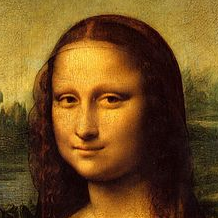
\includegraphics[width=2in]{alsing0.png}\qquad
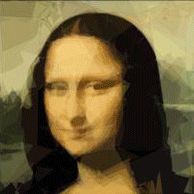
\includegraphics[width=2in]{alsing1.png}
\caption{Genetic Programming: Evolution of Mona Lisa, by Roger Alsing, the original inspiration for the project. The image on the left is a section of the original Mona Lisa painting, and the image on the right is the evolved image constructed with 50 transparent polygons. \cite{alsing}}
\label{jpegfig}
\end{center}
\end{figure*}

\begin{figure*}[!htb]
\begin{center}
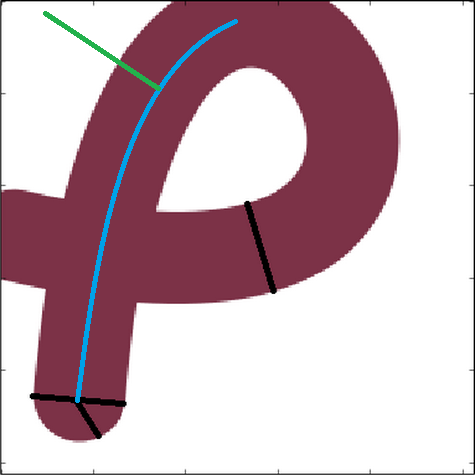
\includegraphics[width=2in]{sample_stroke.png}\qquad
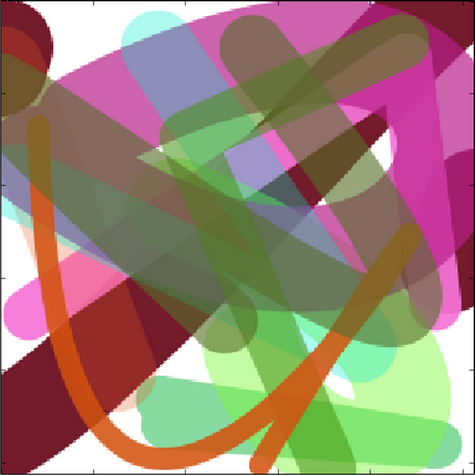
\includegraphics[width=2in]{sample_image.png}
\caption{Sample Stroke and Image: The image on the left shows a random stroke, with the black lines measuring the width of the stroke. The blue line is a segment of the spline curve, and the green line shows the shortest distance between a single pixel and the spline. The shortest distance to the spline must be computed for every pixel to the spline (Hausdorff metric) to explicitly render the stroke. The image on the right is a sample image with a set of random strokes upon initialization.}
\label{jpegfig}
\end{center}
\end{figure*}

\section{The Genetic Painter}
The core of our project is to implement an image painter that evolves images using a genetic algorithm. The change from Alsing's implementation is that our image building blocks are actual brush strokes, which we believe are the intuitive "building blocks" for images as paintings in particular. Additionally, the use of brush strokes was also chosen in order to achieve the desired "Impressionist" style of painting.

We note that although a reasonable result was produced in Alsing's experiment, a significant amount of time was used (over 900,000 generations), most likely due to the lack of crossovers and a limited population size. As such, we were confident that by replacing polygons with brush strokes, we would be able to achieve a similar result at the very least. Consider that if we simply each brush stroke to two points and a stroke width, the strokes are effectively rectangles and hence a decent result can be expected.

In other derivative works, more "proper" genetic algorithim approaches were taken such as accounting for adjustable population size, selection, DNA mixing, etc., and the approaches were able to achieve a faster convergence to the work of the Mona Lisa. However, the authors did not benchmark the amount of time necessary for a visually undiscernible image to the original to be generated. These works demonstrate our belief that adding crossovers and other improvements will result in faster convergence then Alsing's straightforward hill-climbing strategy.

Finally, we would like to note that in contrast to these works we will not be mutating polygons, which causes differences in distribution of the space covered in the image. For example, even when using up to 4 to 5 points per spline, the space that we cover may be rather thin and limited. Essentially, the point while the focus of the problem remains similar, the problem space is extremely different and is presumably more difficult to evolve.

\section{Modeling Paintings and Brush Strokes}

Our general approach was to create a set of strokes $s$, each are composed by splines with $k$ points, $h$ hue, $o$ opacity, and $t$ thickness. The strokes would undergo the process of evolution as dictated by the genetic algorithm which would ultimately result in a set of improved strokes $\hat{s}$ that would resemble the original image.

\subsection{Genome}
The bottom-most representation of the genenome in this work was the stroke. The genes contained a list of points with x, y coordinates, determining each location of the sequential points for the spline curve. The number of spine points is restricted to be at least 2 (a line) than 2 but no greater than 5. We limited the number of points to be less than 5 to avoid resulting in a stroke that covered the entire image. All the points were generated via a random uniform distribution whose ranges were capped by the maximum width and maximum height of the image. Additionally, the gene contained information about the color in the standard RGB format with a range of integer values of 0 to 255 for each color. All 3 channels had their values generated initially via a random uniform distribution. To deal with the problem of layering strokes, each stroke was also assigned an alpha value to add the factor of opacity into the painting. The alpha value was contained between the values of 0.25 and 1.0. The alpha value was also generated initially via a random uniform distribution. Finally, to account for the width of the stroke, a width factor was included in the stroke. To avoid drawing too thin or too wide, the width of the stroke was generate uniformly between 5 to 15 percent of the minimum of the height and width of the image.

\subsection{Population and Survival Policy}
Unlike the Alsing work, we choose to keep both an adjustable population of adults and children. In our tests with a 256 x 256 image, we used population sizes ranging from 30 to 100 for both children and for the parents. In addition, we added a survival policy to recently mutated children to give them a competitive advantage in the testing. That is, some children, regardless of fitness, are spared from the filtering process for an adjustable period of rounds. The intuition behind employing such a policy was to prevent our program from dropping into a local minimum. The only disadvantage of the policy is the sacrificed additional resources that are necessary to keep the less fit offspring alive and allowing them to reproduce.

\subsection{Mutation}
We incorporate multiple levels of mutation to provide for the maximum level of adjustability. At the highest level, we have that each gene which is a stroke can be mutated via addition, editing, or deletion. In the case of addition which has an adjustable rate parameter, we append a completely random new stroke based on the same initial generation parameters to the DNA sequence. Given the opacity parameters, the ordering should not matter. In the case of deletion, we can choose to delete one of the genes or strokes completely from the sequence. Finally, in the case of editing, we can choose to replace the gene with a completely new gene, i.e. addition and deletion combined.
However, we note the mutation for editing may be too drastic and hence, we have a separate level of mutations. Instead of simply changing the entire stroke, we mutate specific attributes of the stroke. This method should prove to be useful when trying to fine tune an image instead of attempting to completely start fresh. We structure the random generation by creating normal distributions centered around the current values for the locations, width, opacity, and color with an adjustable standard deviation. Essentially, instead of randomly guessing with no bias, we attempt to shift the stroke slightly and see if we can find any improvements nearby. Additionally, in this case, we can also choose to remove or add points in the spline of the stroke.

\subsection{Crossovers}
The crossoveres of the DNA were implemented in a couple of methods.

First, the most naive method we chose to use was to pick two DNA strands and we uniformly randomly picked genes or strokes from both strands. Additionally, we pick one strand randomly over the other to determine the length of the strand. However, we expect such a method to yield a random data that does not significantly improve the result. That is, given that a group of strokes together are what most likely cause the fitness to do well as a whole, removing one of these from the group or merging two groups will not necessarily improve the fitness unless they are a large mutually exclusive set.

The other approach we attempt is to swap out entire regions from the DNA strand in an attempt to transfer entire groups of strokes that work well together.
We present the pseudo-code in the next section.

\section{Image Similarity}
The $L_1$-norm and the $L_2$-norm errors are used to evaluate image similarity between two images. Given image A and image B, the fitness function for the $L_1$-norm variant would be defined as
\[ \sum\limits_{i,j} |A_{i,j} - B_{i,j}| \]
which intuitively means that the fitness function accounts for total absolute error between two images, equally weighting the color offset for each pixel.
For a fitness function of the $L_2$-norm error, we have
\[ \sum\limits_{i,j} (A_{i,j} - B_{i,j})^2 \]
which puts greater weights on larger pixel offsets. While we did try using both metrics for evaluating similarity, we can intuitively see why most image processing algorithms use the $L_2$-norm. Instead of weighting all offsets equally, larger outliers are more heavily penalized. For example, an image that is consistently off by one shade of red throughout the entire image is preferable to an image that has a large color offset for a small region of the image. The idea is that optimizing for error in the $L_2$-norm preserves the salient features of the source image and is appropriate when a one-to-one mapping exists between pixels of the sample and source images. Additionally, the $L_2$-norm and RMSE as used in our application is similar to peak signal-to-noise ratio, which evaluates the accuracy of a lossy method for reconstructing signals. Other image similarity metrics were considered, such as normalized color histograms, but the focus was mostly on the implementing and refining our model.

\section{Image Rendering}
We explored various methods of rendering the complete image from a list of stroke genomes. The original method was, for every given point in the image, determine the closest point on each and every spline curve to the point using the methods detailed by Wang et. al \cite{wang}. Using this distance and the width of the spline, we can determine whether the pixel would have been covered by a certain spline. In essence, we are computing the Hausdorff metric between the space of pixels on the image and the points on the spline curve. In our implementation, we determined that an image of 100 splines and size 256 x 256, took approximately 3 seconds on an Intel  4.4Ghz i-3570k processor. Further testing yielded that the bottleneck factor was not the $L_2$-norm being computed but rather the actual rendering of the spline. In essence, for an image of size $MN$ with $K$ splines, it required $MNK$ iterations of the composite Newton method described in the paper. For our purposes, the rendering was drastically too slow to generate any reasonable number of generations in the the project time frame, with each generation taking over a minute to compute. We also explored image downsampling techniques, which are outlined in the following section.

The next approach to achieve rendering in a computatably feasible manner was to draw the splines and then morphologically dilate the pixels of the spline. While the method appears to have the same worst case performance, we achieved some speedup, although the overall computation was still too slow. Finally we used a rendering aggregator to still , the rendering was achieved in approximately 0.01 seconds. Specifically, we chose to use the $RenderAgg$ package from the matplotlib python library. We deemed that this computation time was sufficient for our purposes.

\section{Image Sampling}
Computing the Hausdorff distance between each spline and each pixel coordinate in the image was too computationally expensive. Thus, we explored computing fitness on a subset of pixels within the evolved and source image as an approximation metric,which lowers the computation costs, since the most expensive step is the fitness computation for each new or mutated image genome. However, in order to accurately sample the image, a subset of $n_p$ pixels that can accurately summarize the salient features within the image is required.

\subsection{Naive Sampling} Two simple approaches are to select $n_p$ pixels in a uniform grid or to select $n_p$ random pixels from the image. However, these methods are inefficient as many of the chosen pixels will be located in homogenous areas without important features. Instead, selecting pixels from edges within the image where the color gradient is changing quickly is more efficient, since those features must be identified to accurately reconstruct the image.  However, simply all the edges is impractical, so we will therefore look for corners, i.e. the points where the edges change the most. The resulting sample set will be the pixels that represent the most change in the image.

\subsection{B-tree Triangular Coding}
To identify the important corners within the image, we implement a popular algorithm used in image compression called binary-tree triangular coding (BTTC), developed by Distasi et al. \cite{distasi}, which recursively decomposes the image into right-angled triangles. The BTTC algorithm represents an image $u$ as a surface $A = \{(x,y,c) | c = u(x,y)\}$.  The goal is to approximate $A$ by a discrete surface $B = \{(x,y,d) | d = G(x,y)\}$ with a finite-set of polyhedrons.  Each polyhedron has a right-angle triangle on the XY plane (PRAT) and an upper face right-angle triangle approximating $A$ (URAT).

As illustration, let $T$ be a PRAT of vertices $P_1 = (x_1,y_1)$, $P_2 = (x_2, y_2)$, and $P_3 = (x_3,y_3)$.  If $c_i = u(x_i,y_i)$, then the $(x_i, y_i, c_i)$ are points in $A$ for $i=\{1,2,3\}$ that define the URAT associated with $T$.  BTTC then approximates $u$ within $T$ with the function $G$ that uses linear interpolation,
\begin{equation}
G(x,y) = c_1 + \alpha(c_2 - c_1) + \beta(c_3 -c_1)
 \label{G}
\end{equation}
where $\alpha$ and $\beta$ are defined as,
$$\alpha = \frac{(x-x_1)(y_3 - y_1) - (y-y_1)(x_3-x_1)}{(x_2-x_1)(y_3 - y_1) - (y_2-y_1)(x_3-x_1)}$$
$$\beta = \frac{(x_2-x_1)(y - y_1) - (y_2-y_1)(x-x_1)}{(x_2-x_1)(y_3 - y_1) - (y_2-y_1)(x_3-x_1)}$$
The approximation has error defined as distance between $u(x,y) \in \mathbb{R}^3$ and $G(x,y)\in \mathbb{R}^3$,
$$\text{err}(x,y) = ||u(x,y) - G(x,y)||_2$$
and we determine if the approximation is sufficient with a error condition based on threshold $\epsilon > 0$,
$$\text{err}(x,y) \leq \epsilon$$

If the condition does not hold for $T$, the PRAT of $T$ is divided into two right-angle triangles.  The subdivision procedure is reiterated until the condition holds for all PRATs, and the resulting structure is a binary-tree where each node represents a triangle with either two or zero children.

The BTTC decomposition requires the image dimensions to be square with edge size $2^m+1$ for some $m$. If the image size is invalid, then each sides are padded by zeros to one plus the next power of two. The runtime complexity for the algorithm is an efficient $O(n \log n)$ for an image with $n$ pixels, and we demonstrate that BTTC is able to accurately choose points in areas of high curvature, since the mean squared error (MSE) is bounded by $\epsilon^2$.  For additional details on the BTTC algorithm, see \cite{distasi}.

\begin{figure*}[!htb]
\begin{center}
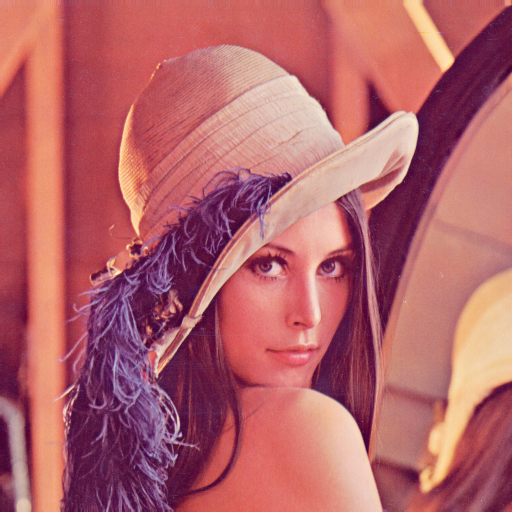
\includegraphics[width=2in]{lena512.png}\qquad
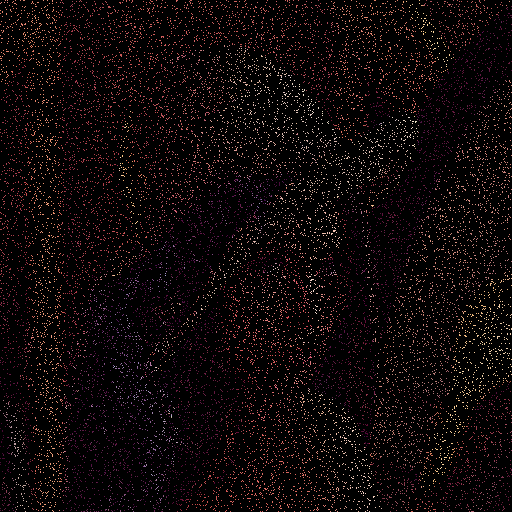
\includegraphics[width=2in]{lena512-random-mask-1.png}\qquad
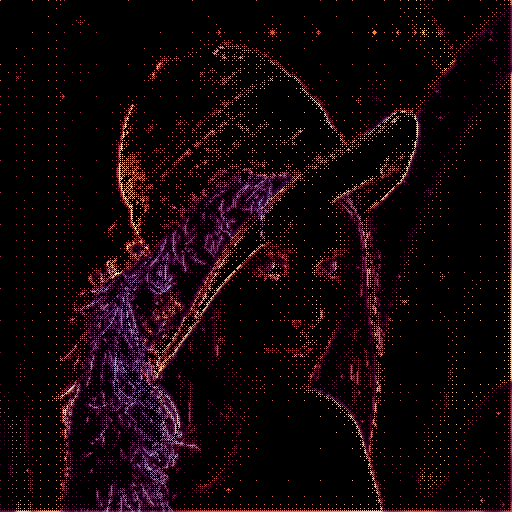
\includegraphics[width=2in]{lena512-bttc-mask-1.png}
\caption{Random vs. BTTC sample selection. For lena512.png, both images are sampled at $\approx 7.62\%$ of the total pixel count. The left image is generated with uniform random sampling. For BTTC on the right, we chose $\epsilon = 0.15$. Note that the BTTC implementation selects dense clusters of points along important edge features in the image, while areas with minor gradients have relatively sparse sampling.}
\label{bttcselectionfig}
\end{center}
\end{figure*}

\subsection{Conclusions}
Creating a sample set of pixels for each source image is inexpensive computationally. The randomized and uniform samples are very fast, but the recursive BTTC algorithm is more complex and depends greatly on the error threshold, although the BTTC tree only needs to be computed once per run. Figure 3 shows a comparison of image sampling with the randomized and BTTC selection methods, and we note that the BTTC algorithm selects pixels that are better represent the salient features of the image.

However, upon further investigation, image downsampling still had serious problems.First, the fitness evaluation is still too slow; a 7 percent sub-sample using the BTTC algorithm essential reduces the new run time to 7 percent of the original run time. With a population of 100 images, a useful number of generations cannot be computed within a reasonable time frame. Additionally, we note that although BTTC should get the most salient pixels of the image, we noticed that areas with sparse sub samples were populated by "junk" brush strokes even though the complex feature areas performed better. Intuitively, we can see why the observation is unsurprising, since the lack of sample pixels means large swaths of inaccurate data could be overlooked.

\section{Implementation}
We detail our actual implementation below.

\subsection{Downsampling}
One of the key limitations that we soon realized was the running time required to generate reasonable results. Hence, given these limitations, it would be computationally infeasible to directly apply genetic algorithms to large pictures. However, we can instead reduce the size of the image to a much smaller level that allows for quick processing. After running the algorithm on the less detailed but similar representation, we can enlarge the image to the next level along with the doubling the sizes of the strokes.

Intuitively, this would allow us to determine the general strokes necessary to produce the key features of the picture quickly. The remaining details which would normally take an exorbitant amount of time to be fine tuned would be done much quicker via a narrowed range of mutation as described above. We detail the pseudo code below.

\subsection{Writing DNA to Files}
One of the core difficulties we encountered was with the duration length of our experiments. That is, due to the computationally intensive manner, we found that our processes would often stall. Moreover, the result of the processing could not be seen until after the trials had finished, limting our ability to test quickly and alter our supervision. To resolve this issue, we chose to write the entire population to a file at each improvement. While this slows the process down due to the File I/O necessary, we believe its utility is worth the cost. We present a sample of our semi-colon delmited format for a single stroke below.

\begin{verbatim}
shape:(128L, 128L);
sx:[ 74.62566933  21.69977093  22.68605165];
sy:[  67.09635735  109.9504711    18.90664948];
color:(0.027076976805653685, 
0.16087405681211719, 
0.14684489042167803);
alpha:0.8511196927;
width:25
\end{verbatim}

\subsection{Gene Pseudo-Code}
\begin{verbatim}
class GeneStroke
  properties
    shape
    spline_xs
    spline_ys
    color
    alpha
    width
\end{verbatim}

\subsection{Population/Survival Policy Pseudo-Code}
\begin{verbatim}
List current_generation
List old_enough
new_mutations = mutate(current_generation)
For dna in current_generations
  If Age(dna) > X
    Add dna to old_enough
  End If
EndFor
survived = Prune old_enough
current_generation = survived + mutations
Increase Age for all dna in current_generation
\end{verbatim}

\subsection{Mutation Pseudo-Code}
\paragraph{DNA Level Mutation}
\begin{verbatim}
Given DNA Strand D
  D_tmp = Clone D
  For gene in D_tmp
    If Random < Probability of Delete or Edit
      If Scaled Random < Cond. Probability of Edit
        gene = new random stroke
      Else
        Delete gene/stroke
      EndIf
    EndIf
  End For
  
  If Random < Probability of Adding Stroke,
    Add New Random Stroke
  EndIf
\end{verbatim}
\paragraph{Gene Level Mutation}
\begin{verbatim}
While nothing mutated
  If Random < Prob mutate color
    Color = Normal(prev value, 0.15,
    				 min_color, max_color)
    Break
  EndIf
  
  If Random < Prob mutate alpha
    Alpha = Normal(prev value, 0.15,
    				 min_alpha, max_alpha)
    Break
  EndIf
  
  If Random < Prob mutate width
    Width = Normal(prev value, 0.15,
    				 min_width, max_width)
    Break
  EndIf
  
  If Random < Prob Add Point
    Append Random Point to Spline
    Break
  EndIf
  
  If Random < Prob Delete Point
    Pick Random Index of Point
    Dlete Spline point at Index
    Break
  EndIf
  
  If Random < Prob Edit Point
  	Pick Random Index of Point
  	point at index =
  	  Normal(prev_value, 0.05*shape,
  	  	0, max_dim)
  	Break
  EndIf

End While
\end{verbatim}

\subsection{Crossover Pseudo-Code}
\begin{verbatim}
Choose random DNA A and random DNA B
For each index in A
  If Random < prob pick
    gene at index in A =
      gene at index for B
  End If
End For
\end{verbatim}

\subsection{Minimal Supervision}
Our minimal supervision implementation uses the following parameters: the number of strokes per DNA strand is 50, a maximum population size of 10, minimum spline points of 2 and a maximum spline points of 3, add mutation rate of 0.2, change or delete mutation rate of 0.07, conditional delete mutation rate of 0.5, a maximum children population of 25, no crossovers, minimum iteration of 50,000. The version employed only DNA level mutations and any sort of mutation resulted in a completely new stroke being generated. We detail the psuedo-code below.

\begin{enumerate}

	\item Generate a set of 10 DNA strands each containing 50 random strokes
	\item Initialize $NumIter$ Counter
	\item While $NumIter < 50000$ And Change In Error in Last 10 rounds is 0
	\item Generate set of 25 mutations
	\item Pick top 10 from the 35 resulting strands
	\item Increment $NumIter$
	\item End While
	\item Output Lowest Error Image

\end{enumerate}

\subsection{Maximal Supervision}
stuff


\section{Experiments}



\section{Results}
\subsection{Minimal Supervision}
\begin{figure*}[!htb]
\begin{center}
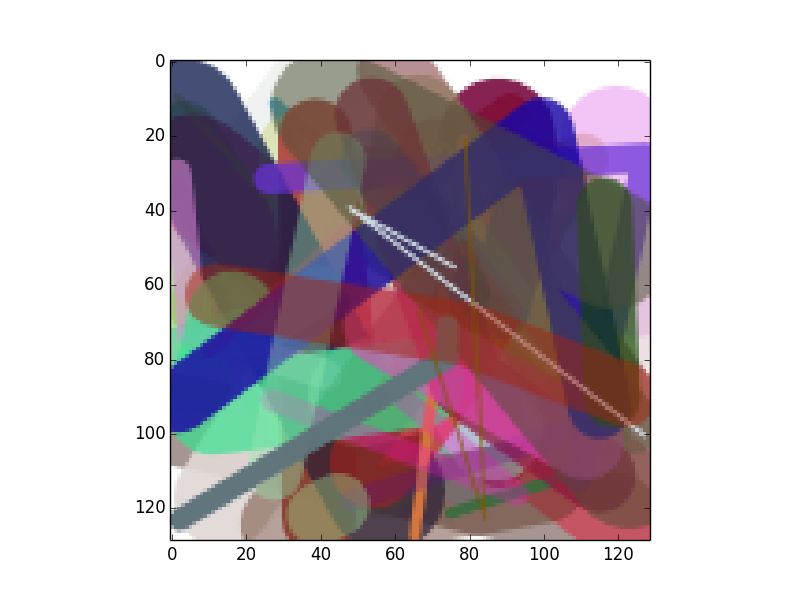
\includegraphics[width=2in]{../groupB/M-1.png}\qquad
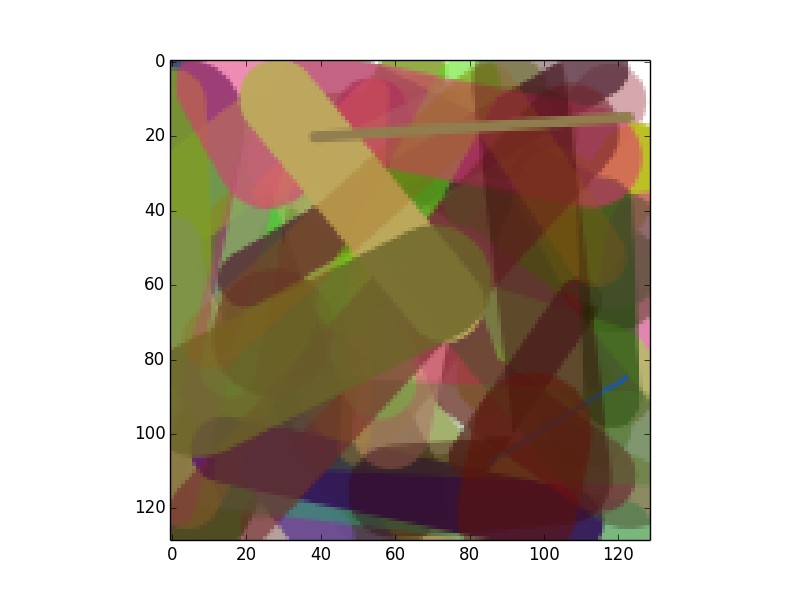
\includegraphics[width=2in]{../groupB/M-200.png}\qquad
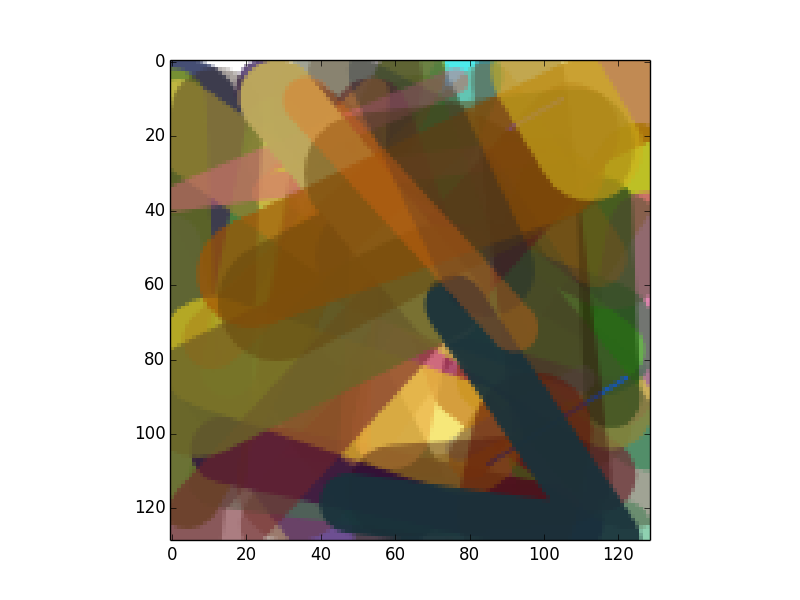
\includegraphics[width=2in]{../groupB/M-424.png}\\
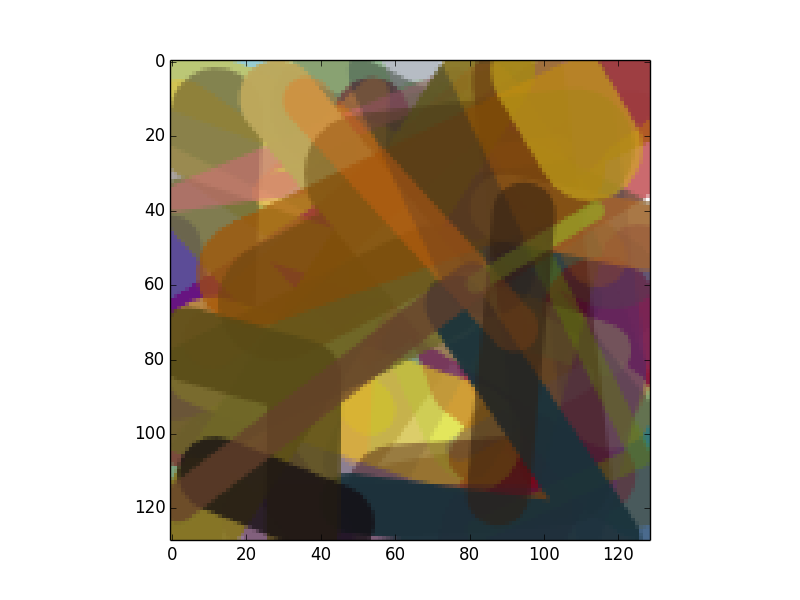
\includegraphics[width=2in]{../groupB/M-1155.png}\qquad
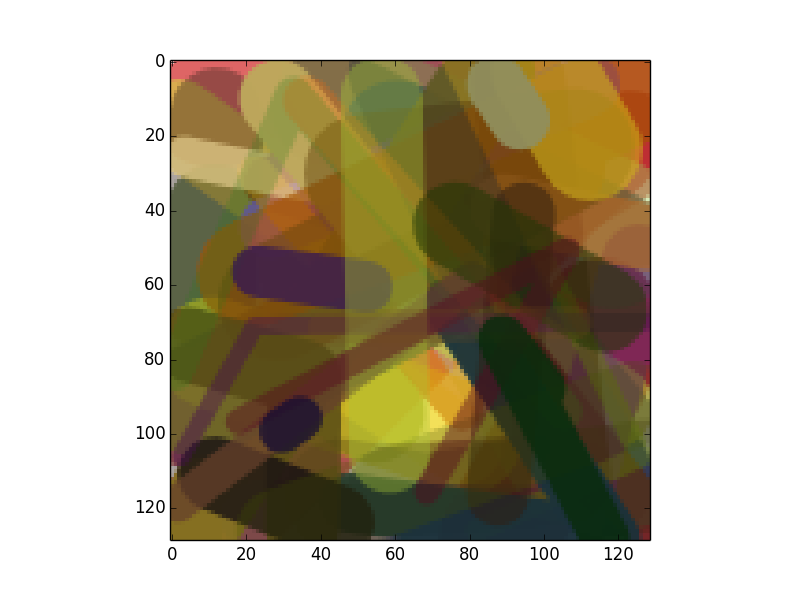
\includegraphics[width=2in]{../groupB/M-2826.png}\qquad
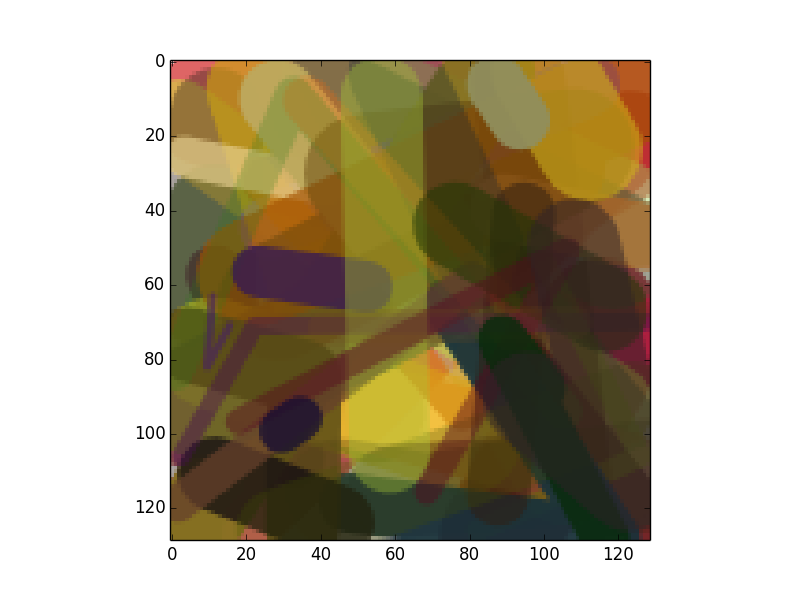
\includegraphics[width=2in]{../groupB/M-3566.png}\\
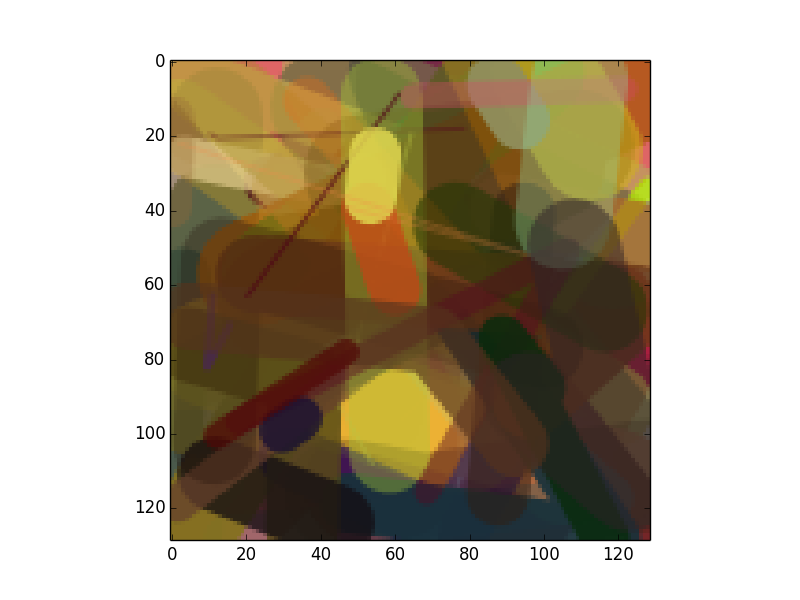
\includegraphics[width=2in]{../groupB/M-11910.png}\qquad
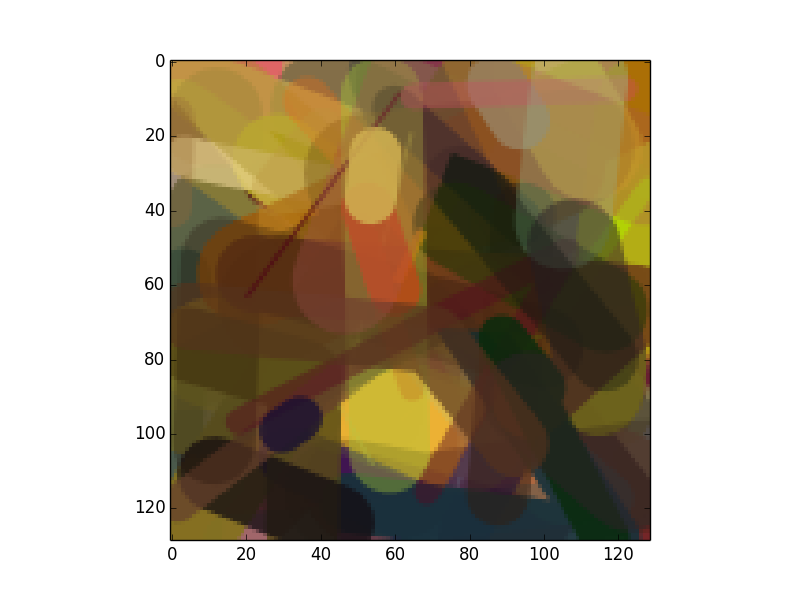
\includegraphics[width=2in]{../groupB/M-14557.png}\qquad
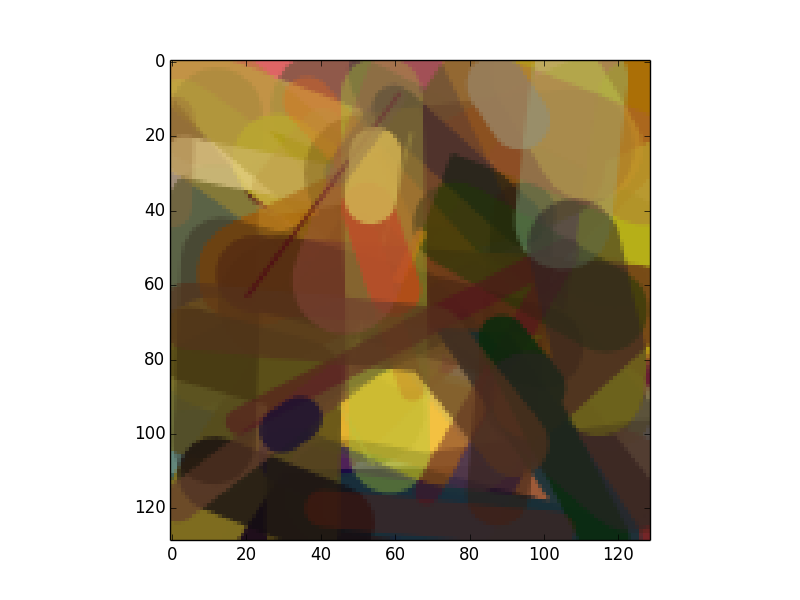
\includegraphics[width=2in]{../groupB/M-16996.png}\\
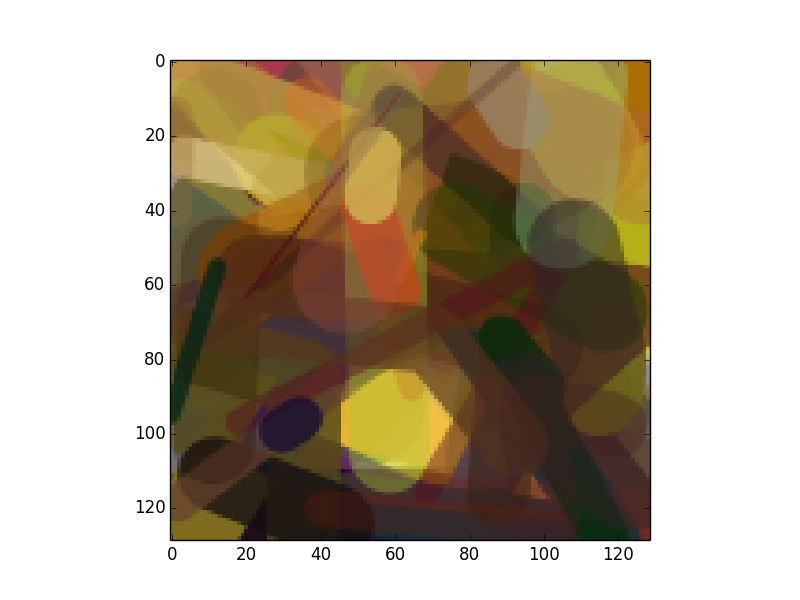
\includegraphics[width=2in]{../groupB/M-21048.png}\qquad
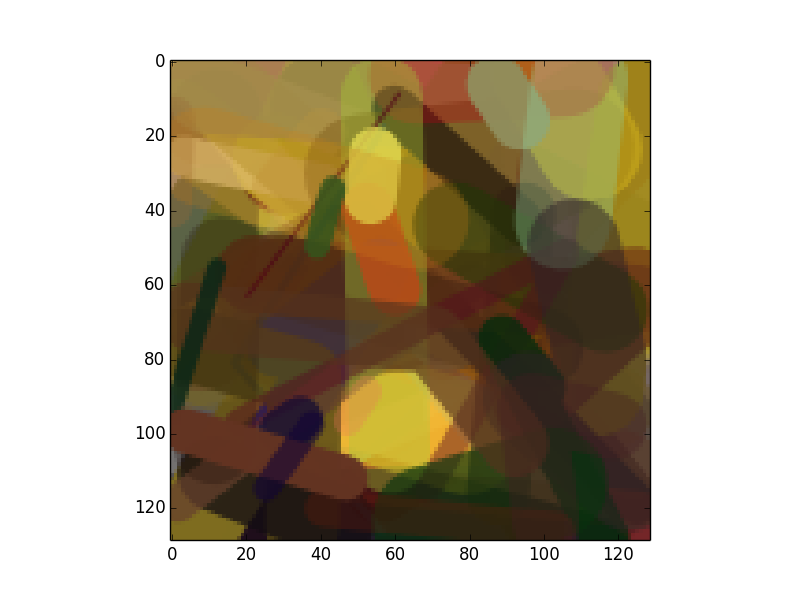
\includegraphics[width=2in]{../groupB/M-37608.png}\qquad
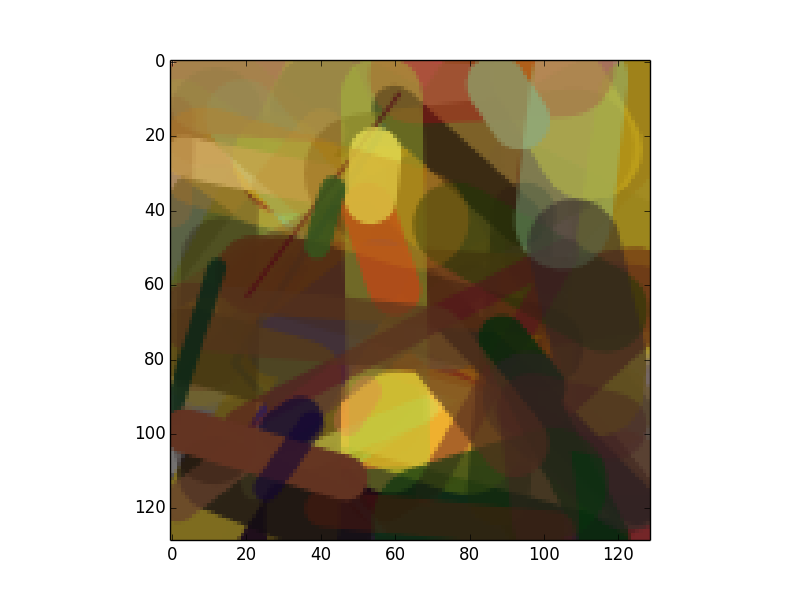
\includegraphics[width=2in]{../groupB/M-42066.png}\\
\caption{Here we have our unsupervised learning genetic algorithm running on the original Mona Lisa image.}
\label{evolutionfig}
\end{center}
\end{figure*}

\pagebreak
\begin{figure*}[!htb]
\begin{center}
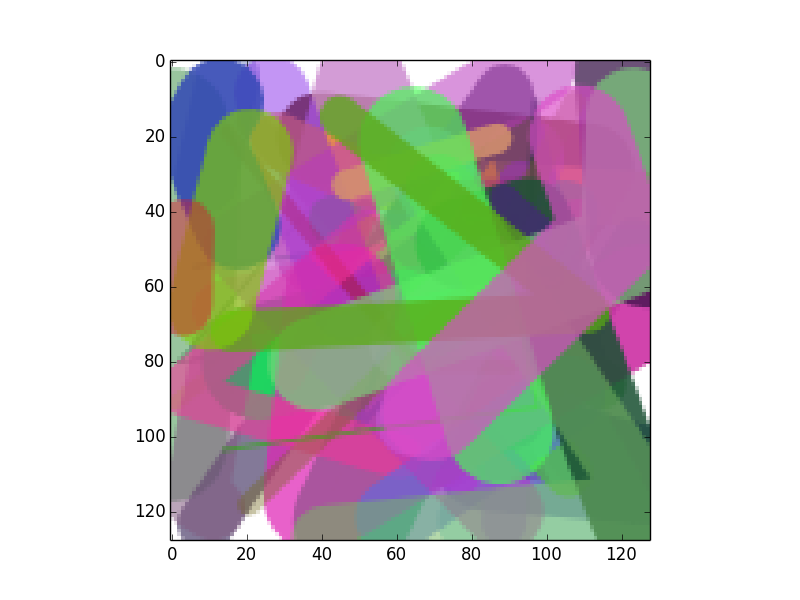
\includegraphics[width=2in]{../groupB/P-1.png}\qquad
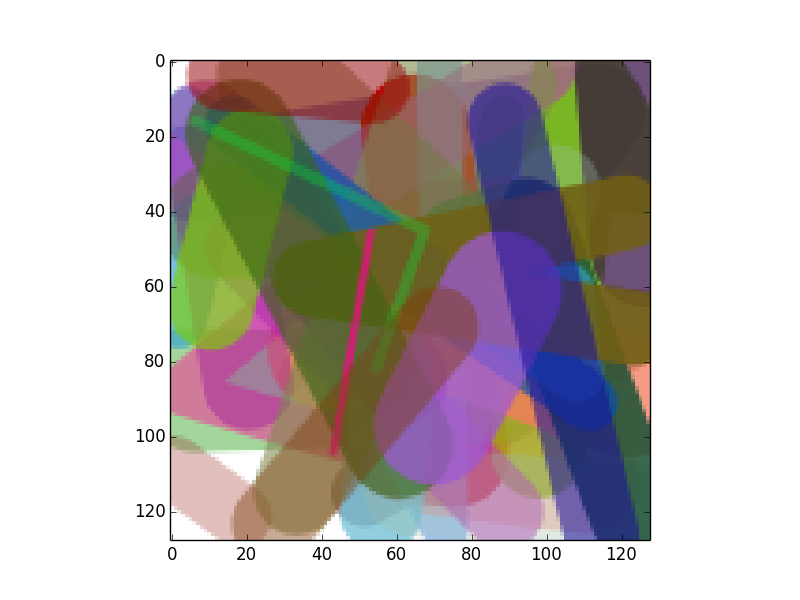
\includegraphics[width=2in]{../groupB/P-28.png}\qquad
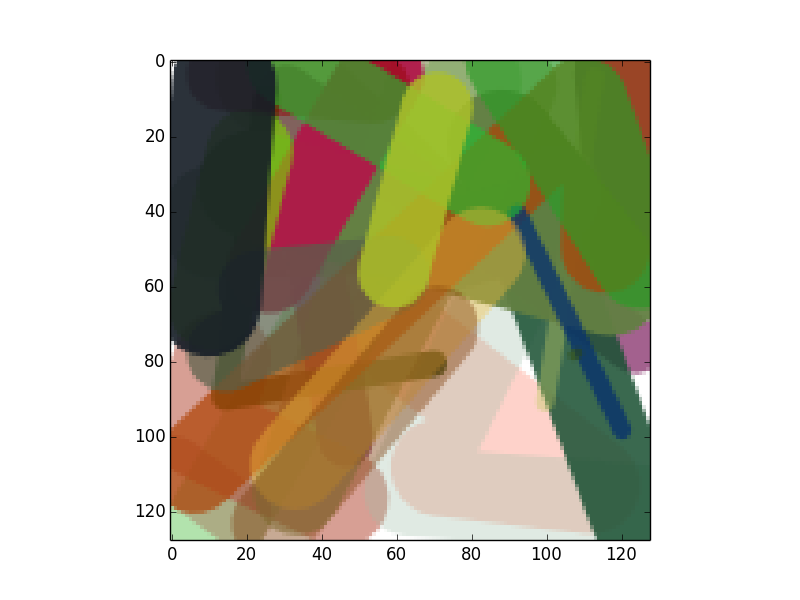
\includegraphics[width=2in]{../groupB/P-117.png}\\
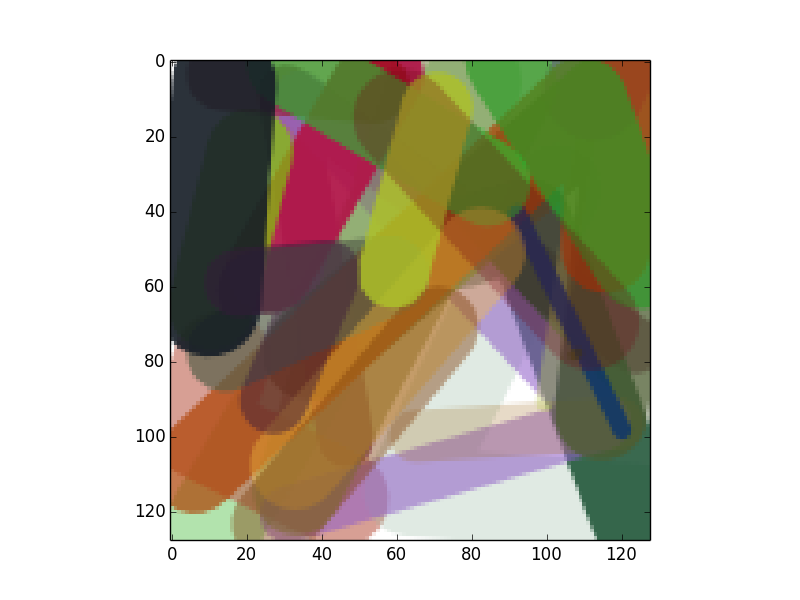
\includegraphics[width=2in]{../groupB/P-192.png}\qquad
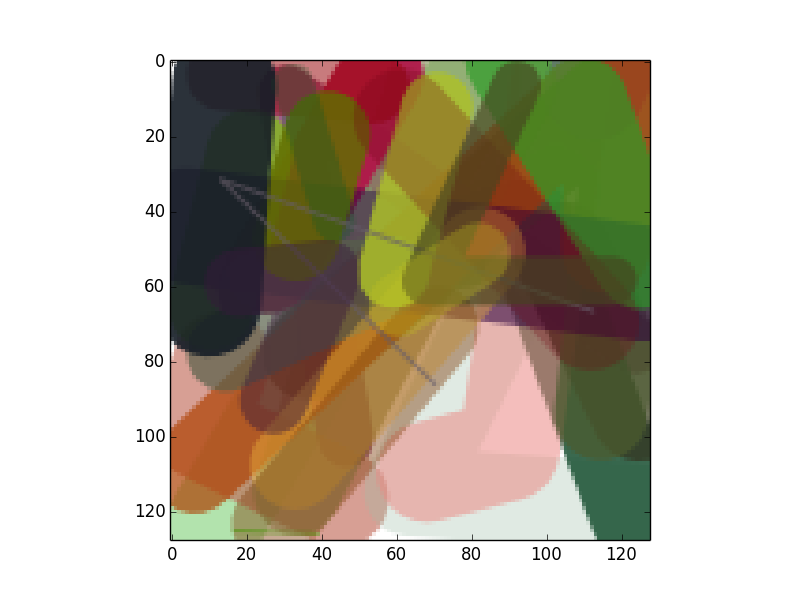
\includegraphics[width=2in]{../groupB/P-286.png}\qquad
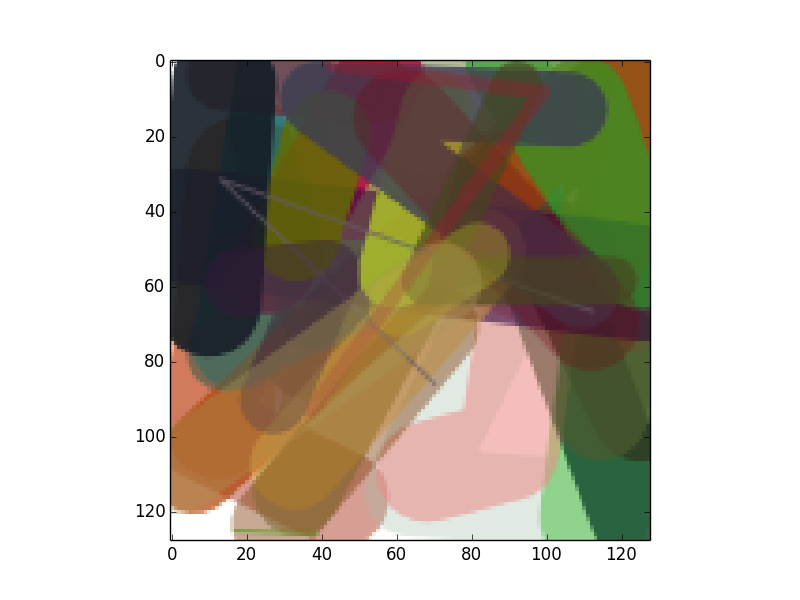
\includegraphics[width=2in]{../groupB/P-412.png}\\
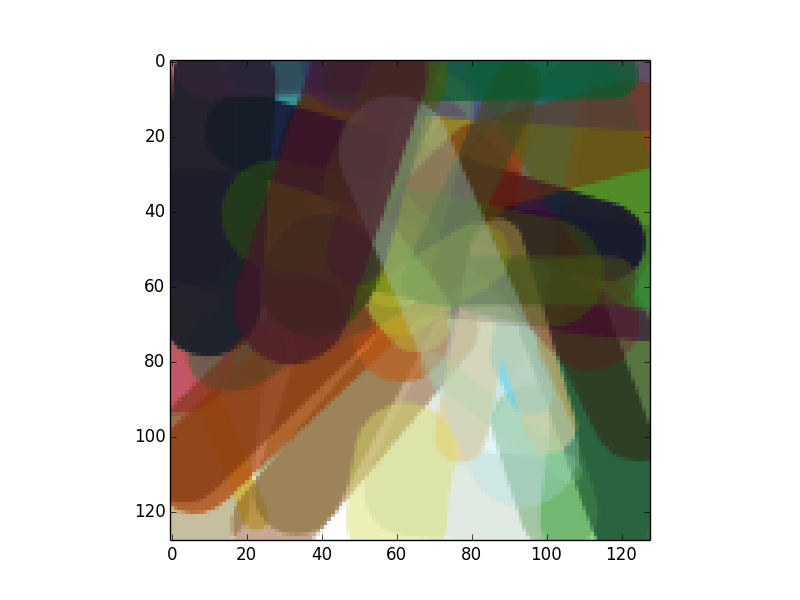
\includegraphics[width=2in]{../groupB/P-1193.png}\qquad
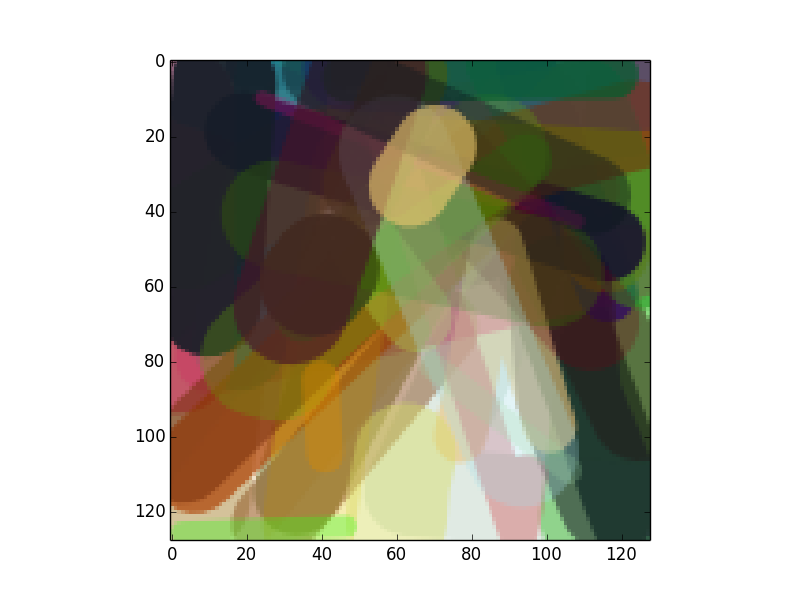
\includegraphics[width=2in]{../groupB/P-2250.png}\qquad
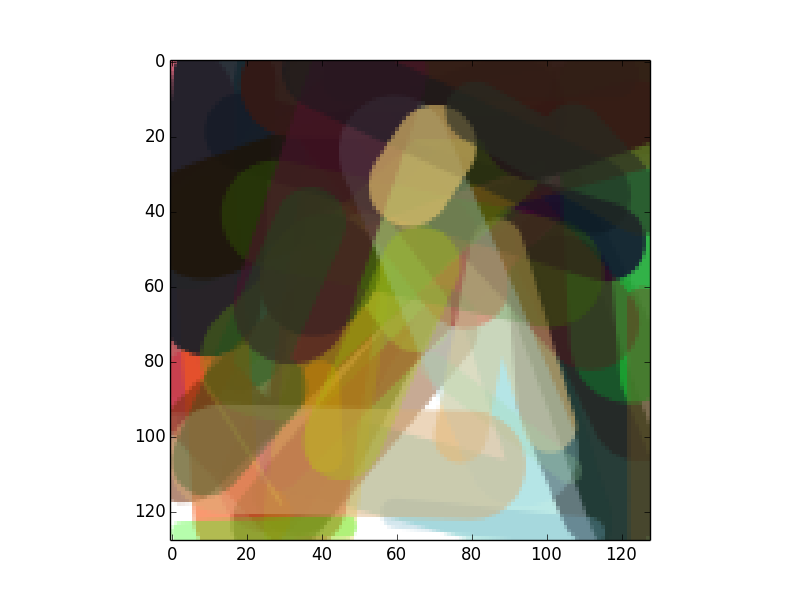
\includegraphics[width=2in]{../groupB/P-3844.png}\\
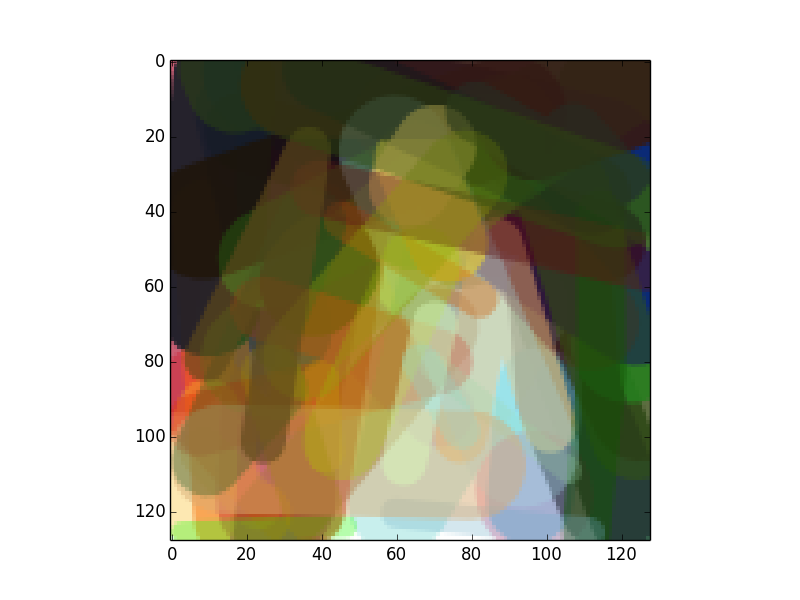
\includegraphics[width=2in]{../groupB/P-10679.png}\qquad
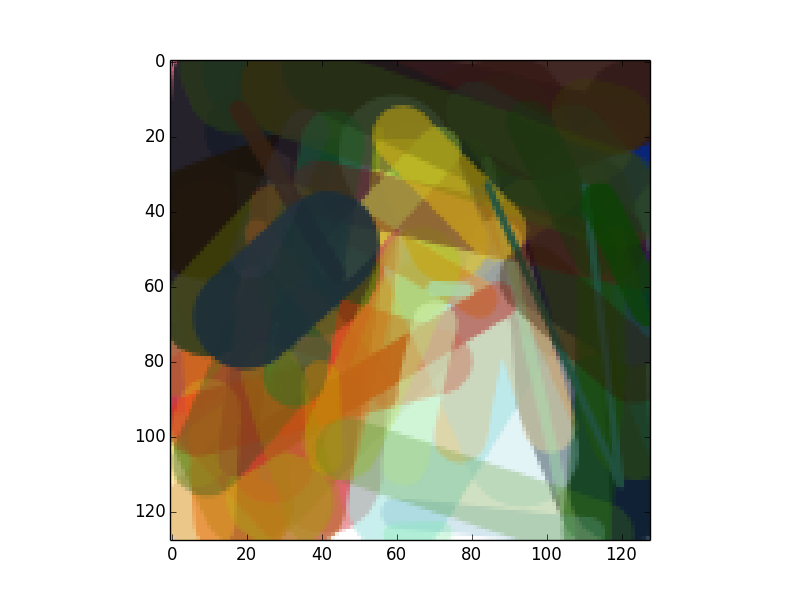
\includegraphics[width=2in]{../groupB/P-39473.png}\qquad
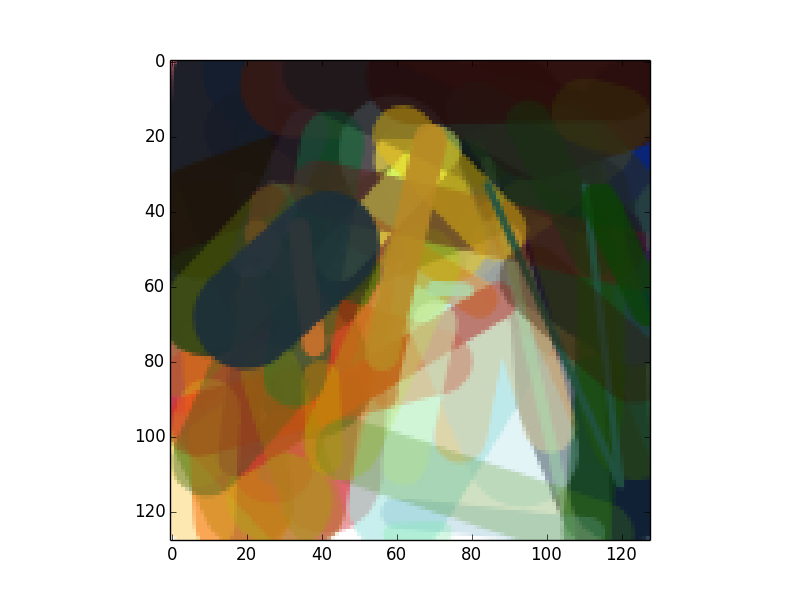
\includegraphics[width=2in]{../groupB/P-42159.png}\\
\caption{Similar to before, we have the supervised learning genetic algorithm running on our Picasso.}
\label{evolutionfig}
\end{center}
\end{figure*}


\subsection{Maximal Supervision}

\begin{figure*}[!htb]
\begin{center}
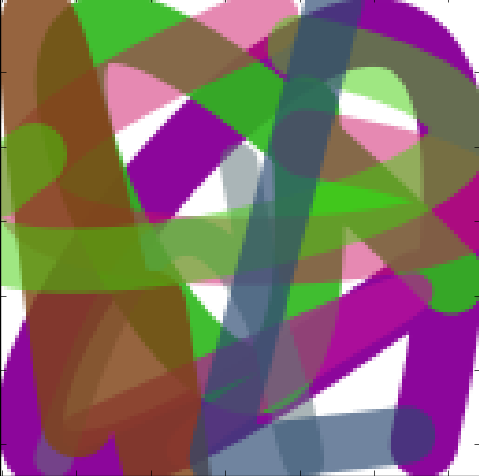
\includegraphics[width=2in]{../groupA/M-102.png}\qquad
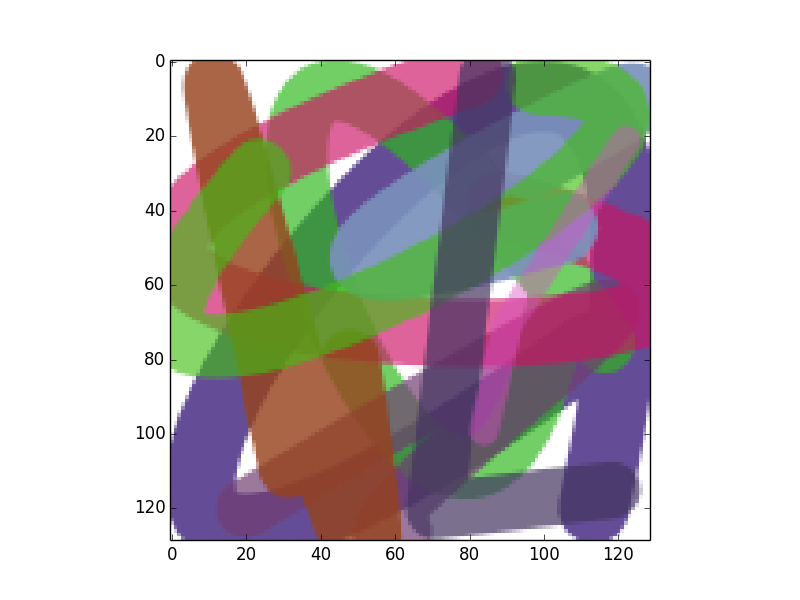
\includegraphics[width=2in]{../groupA/M-156.png}\qquad
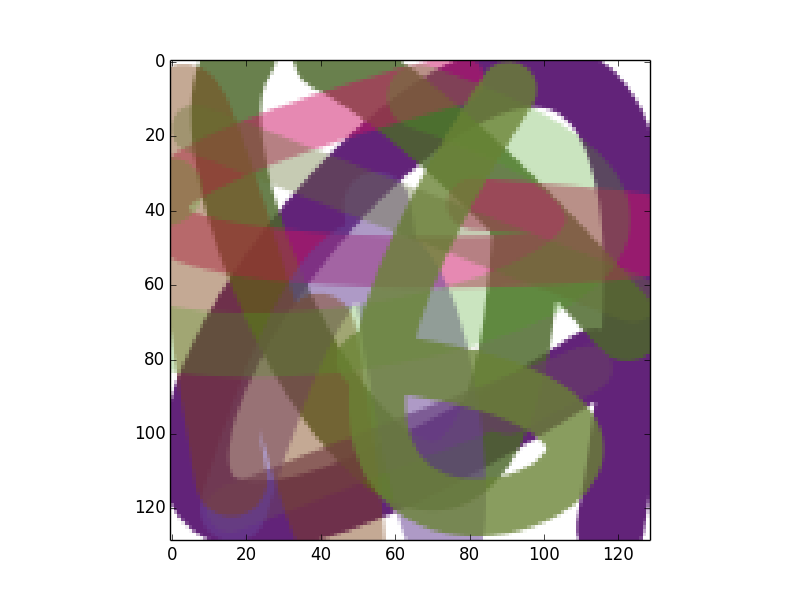
\includegraphics[width=2in]{../groupA/M-288.png}\\
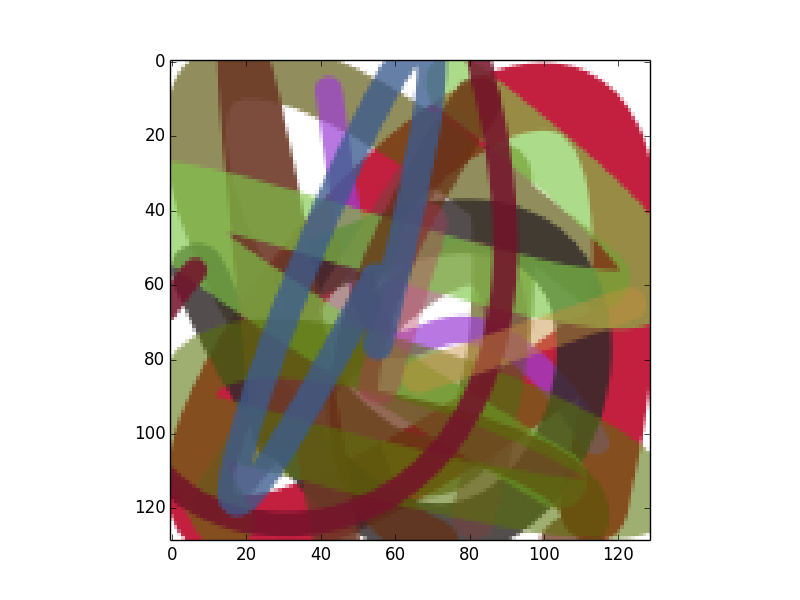
\includegraphics[width=2in]{../groupA/M-427.png}\qquad

\includegraphics[width=2in]{../groupA/M-515.png}\qquad

\includegraphics[width=2in]{../groupA/M-1161.png}\\
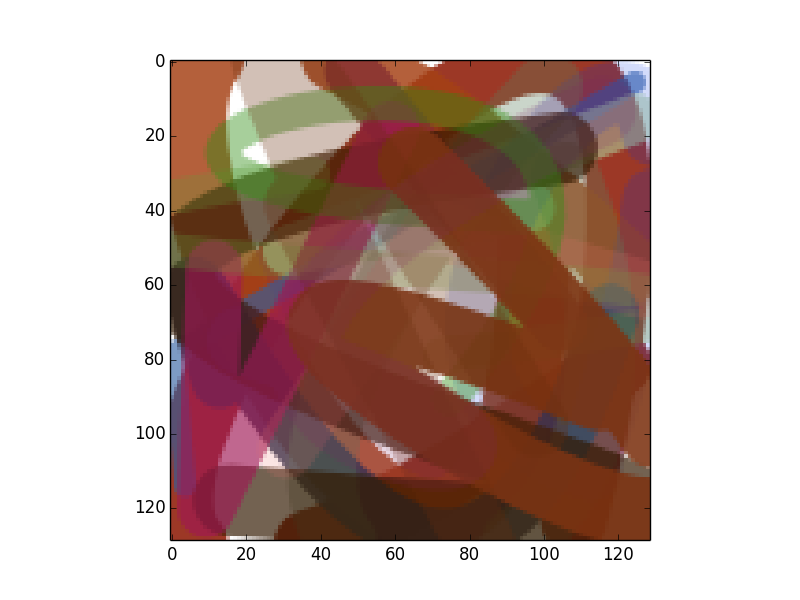
\includegraphics[width=2in]{../groupA/M-1813.png}\qquad
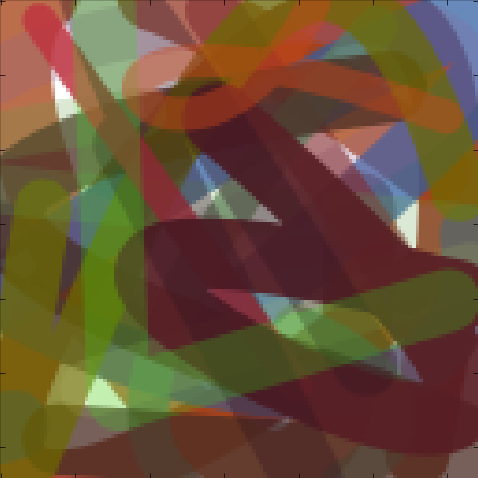
\includegraphics[width=2in]{../groupA/M-3178.png}\qquad
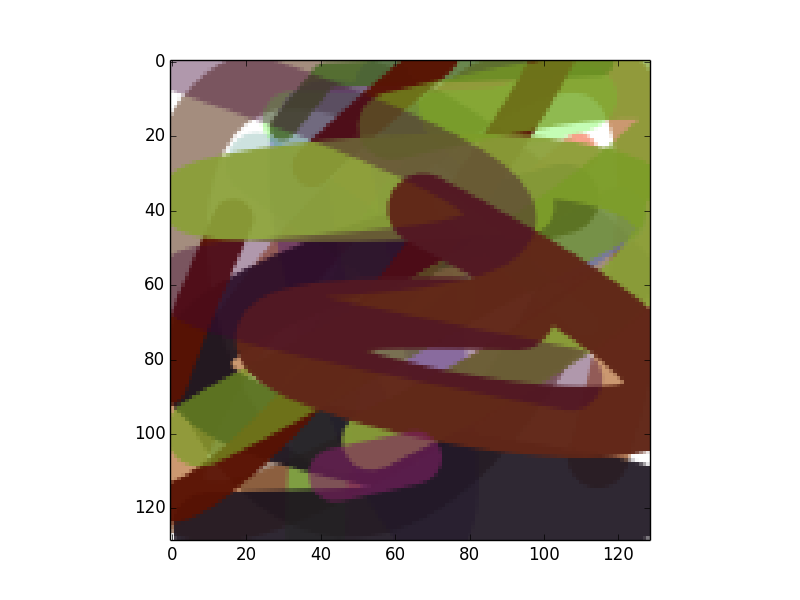
\includegraphics[width=2in]{../groupA/M-4578.png}\\
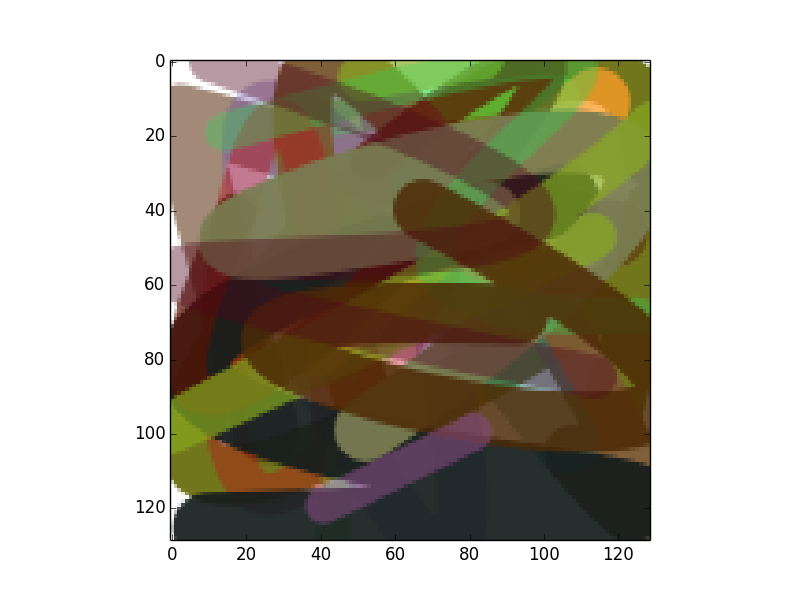
\includegraphics[width=2in]{../groupA/M-14630.png}\qquad
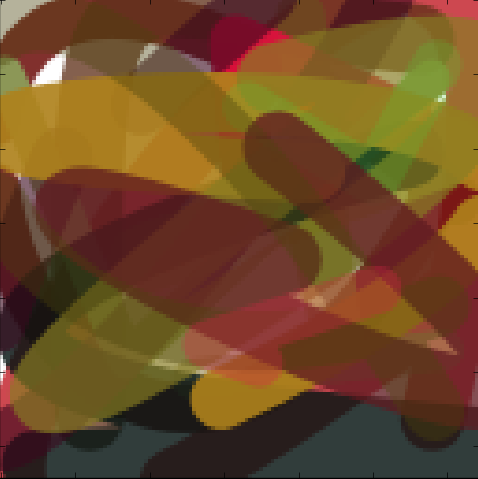
\includegraphics[width=2in]{../groupA/M-35131.png}\qquad
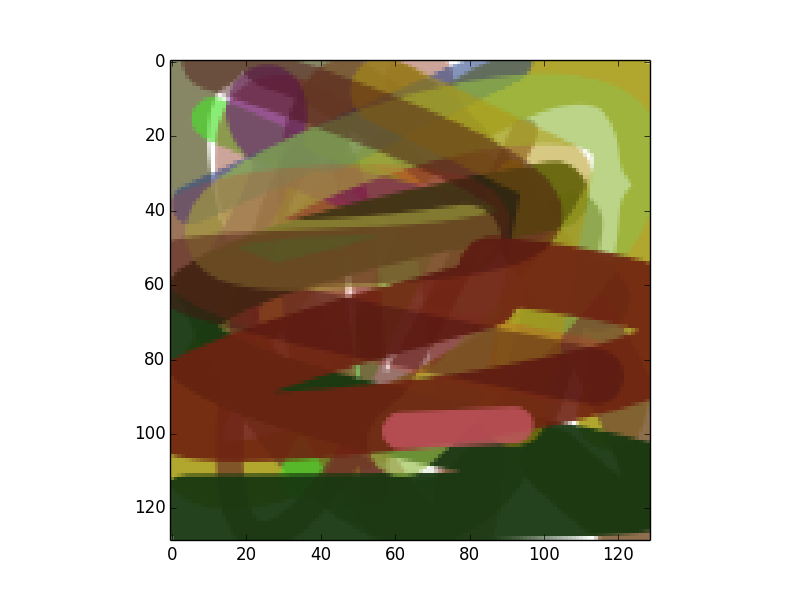
\includegraphics[width=2in]{../groupA/M-36522.png}\\
\caption{Here we have our supervised learning genetic algorithm running on the original Mona Lisa image.}
\label{evolutionfig}
\end{center}
\end{figure*}

\pagebreak
\begin{figure*}[!htb]
\begin{center}
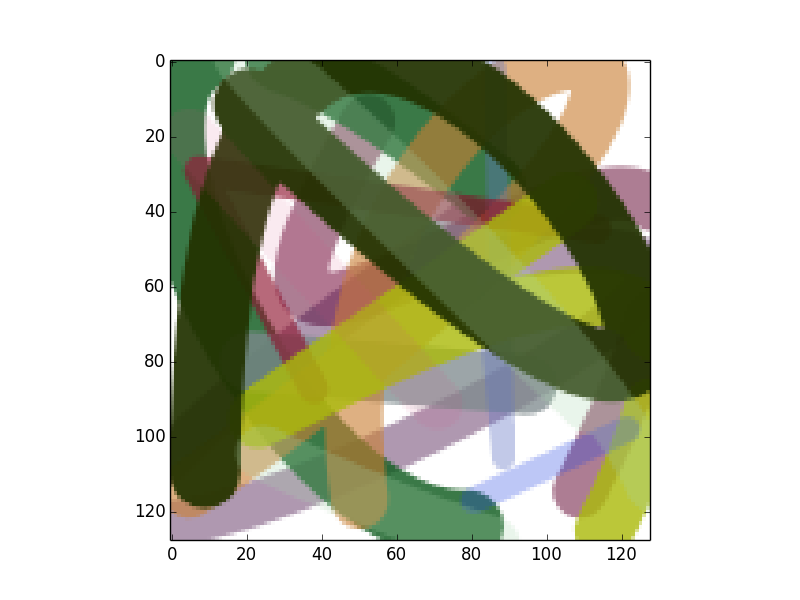
\includegraphics[width=2in]{../groupA/P-126.png}\qquad
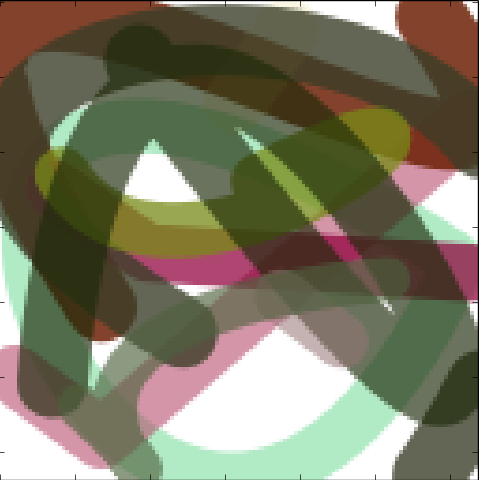
\includegraphics[width=2in]{../groupA/P-199.png}\qquad
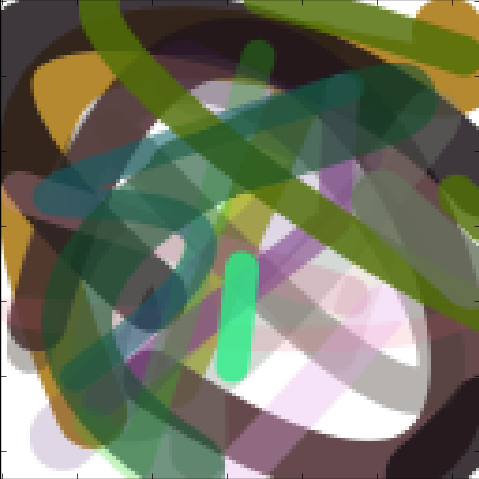
\includegraphics[width=2in]{../groupA/P-629.png}\\
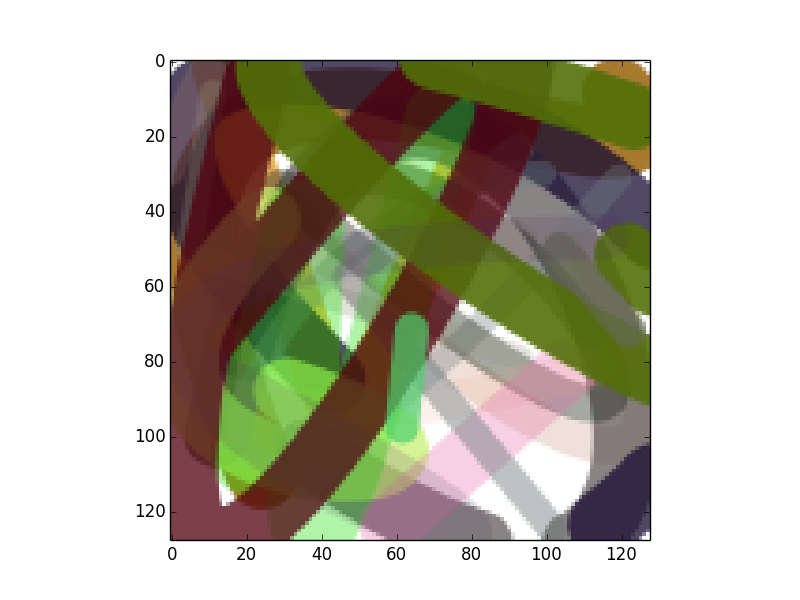
\includegraphics[width=2in]{../groupA/P-1416.png}\qquad
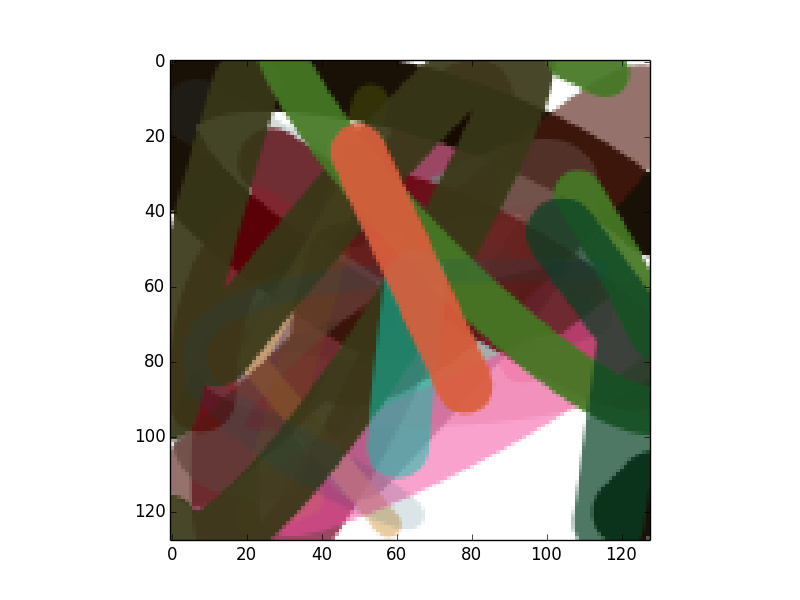
\includegraphics[width=2in]{../groupA/P-1889.png}\qquad
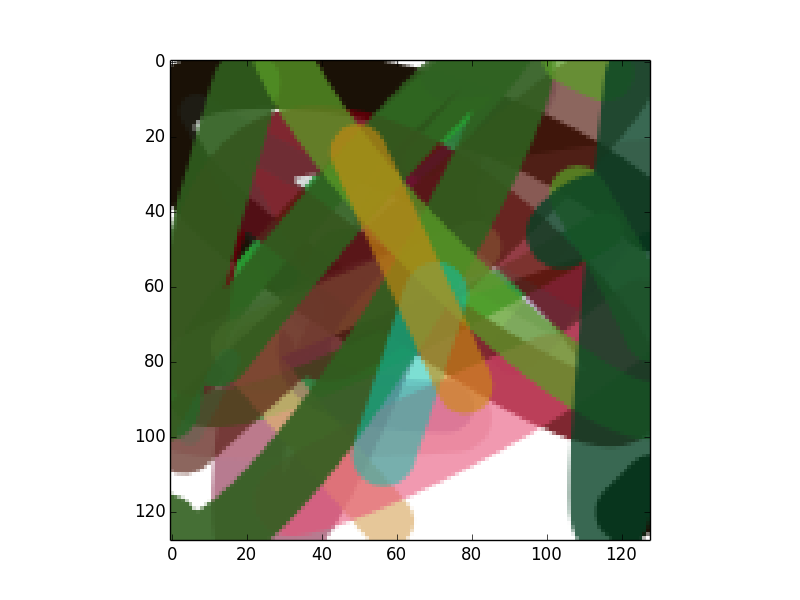
\includegraphics[width=2in]{../groupA/P-3921.png}\\
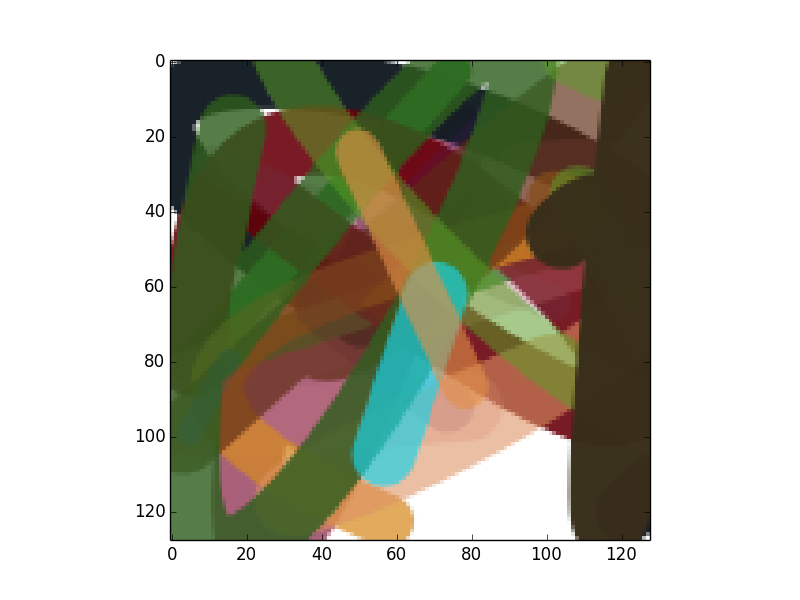
\includegraphics[width=2in]{../groupA/P-4321.png}\qquad
\includegraphics[width=2in]{../groupA/P-6558.png}\qquad
\includegraphics[width=2in]{../groupA/P-7792.png}\\
\includegraphics[width=2in]{../groupA/P-8391.png}\qquad
\includegraphics[width=2in]{../groupA/P-14741.png}\qquad
\includegraphics[width=2in]{../groupA/P-49320.png}\\
\caption{Similar to before, we have the supervised learning genetic algorithm running on our Picasso.}
\label{evolutionfig}
\end{center}
\end{figure*}

\section{Conclusion}
asdf

\begin{thebibliography}{10}

\bibitem{alsing}
Roger Alsing, {\em Genetic Programming: Evolution of Mona Lisa}, http://rogeralsing.com/2008/12/07/genetic-programming-evolution-of-mona-lisa/.

\bibitem{wang}
Hongling Wang, Joseph Kearney, and Kendall Atkinson, {\em Robust and Efficient Computation of the Closest Point on a Spline Curve}, Dept. of Computer Science, The University of Iowa, (2002).

\bibitem{distasi}
R.~Distasi, M.~Nappi, and S.~Virtulano, {\em Image Compression by {BTTC}-Tree Triangular Coding}, IEEE Transactions on Communication, 45, 9 (1997).

\end{thebibliography}

%----------------------------------------------------------------------------------------

\end{article}

\end{document}